% 请确保文件编码为utf-8,使用XeLaTex进行编译,或者通过overleaf进行编译

\documentclass[answers]{exam}  % 使用此行带有作答模块
% \documentclass{exam} % 使用此行只显示题目

\usepackage{xeCJK}
\usepackage{zhnumber}
\usepackage{graphicx}
\usepackage{hyperref}
\usepackage{amsmath}
\usepackage{amssymb}
\usepackage{mathtools}
\usepackage{booktabs}
\usepackage{enumerate}
\usepackage{ctex}


\title{2024秋季高级机器学习 \\ 习题三}
\date{2024.12.12}
\pagestyle{headandfoot}
\firstpageheadrule
\firstpageheader{南京大学}{2024秋季高级机器学习}{习题三}
\runningheader{南京大学}
{2024秋季高级机器学习}
{习题三}
\runningheadrule
\firstpagefooter{}{第\thepage\ 页(共\numpages 页)}{}
\runningfooter{}{第\thepage\ 页(共\numpages 页)}{}
\author{221300079 王俊童}
% no box for solutions
% \unframedsolutions

\setlength\linefillheight{.5in}

% \renewcommand{\solutiontitle}{\noindent\textbf{答:}}
\renewcommand{\solutiontitle}{\noindent\textbf{解:}\par\noindent}

\renewcommand{\thequestion}{\zhnum{question}}
\renewcommand{\questionlabel}{\thequestion .}
\renewcommand{\thepartno}{\arabic{partno}}
\renewcommand{\partlabel}{\thepartno .}

\def\dist{{\mathrm{dist}}}
\def\x{{\boldsymbol{x}}}
\def\w{{\boldsymbol{w}}}


\begin{document}
% \normalsize
\maketitle

\begin{questions}

\question [40] \textbf{概率图模型}

\begin{parts}

 \part [20] 
     图~\ref{fig:dag}是一个贝叶斯网络结构,请仿照教材14.4.1变量消去部分内容,推断图中边际概率$P(x_5)$.
    \begin{figure}[hp]
    \centerline{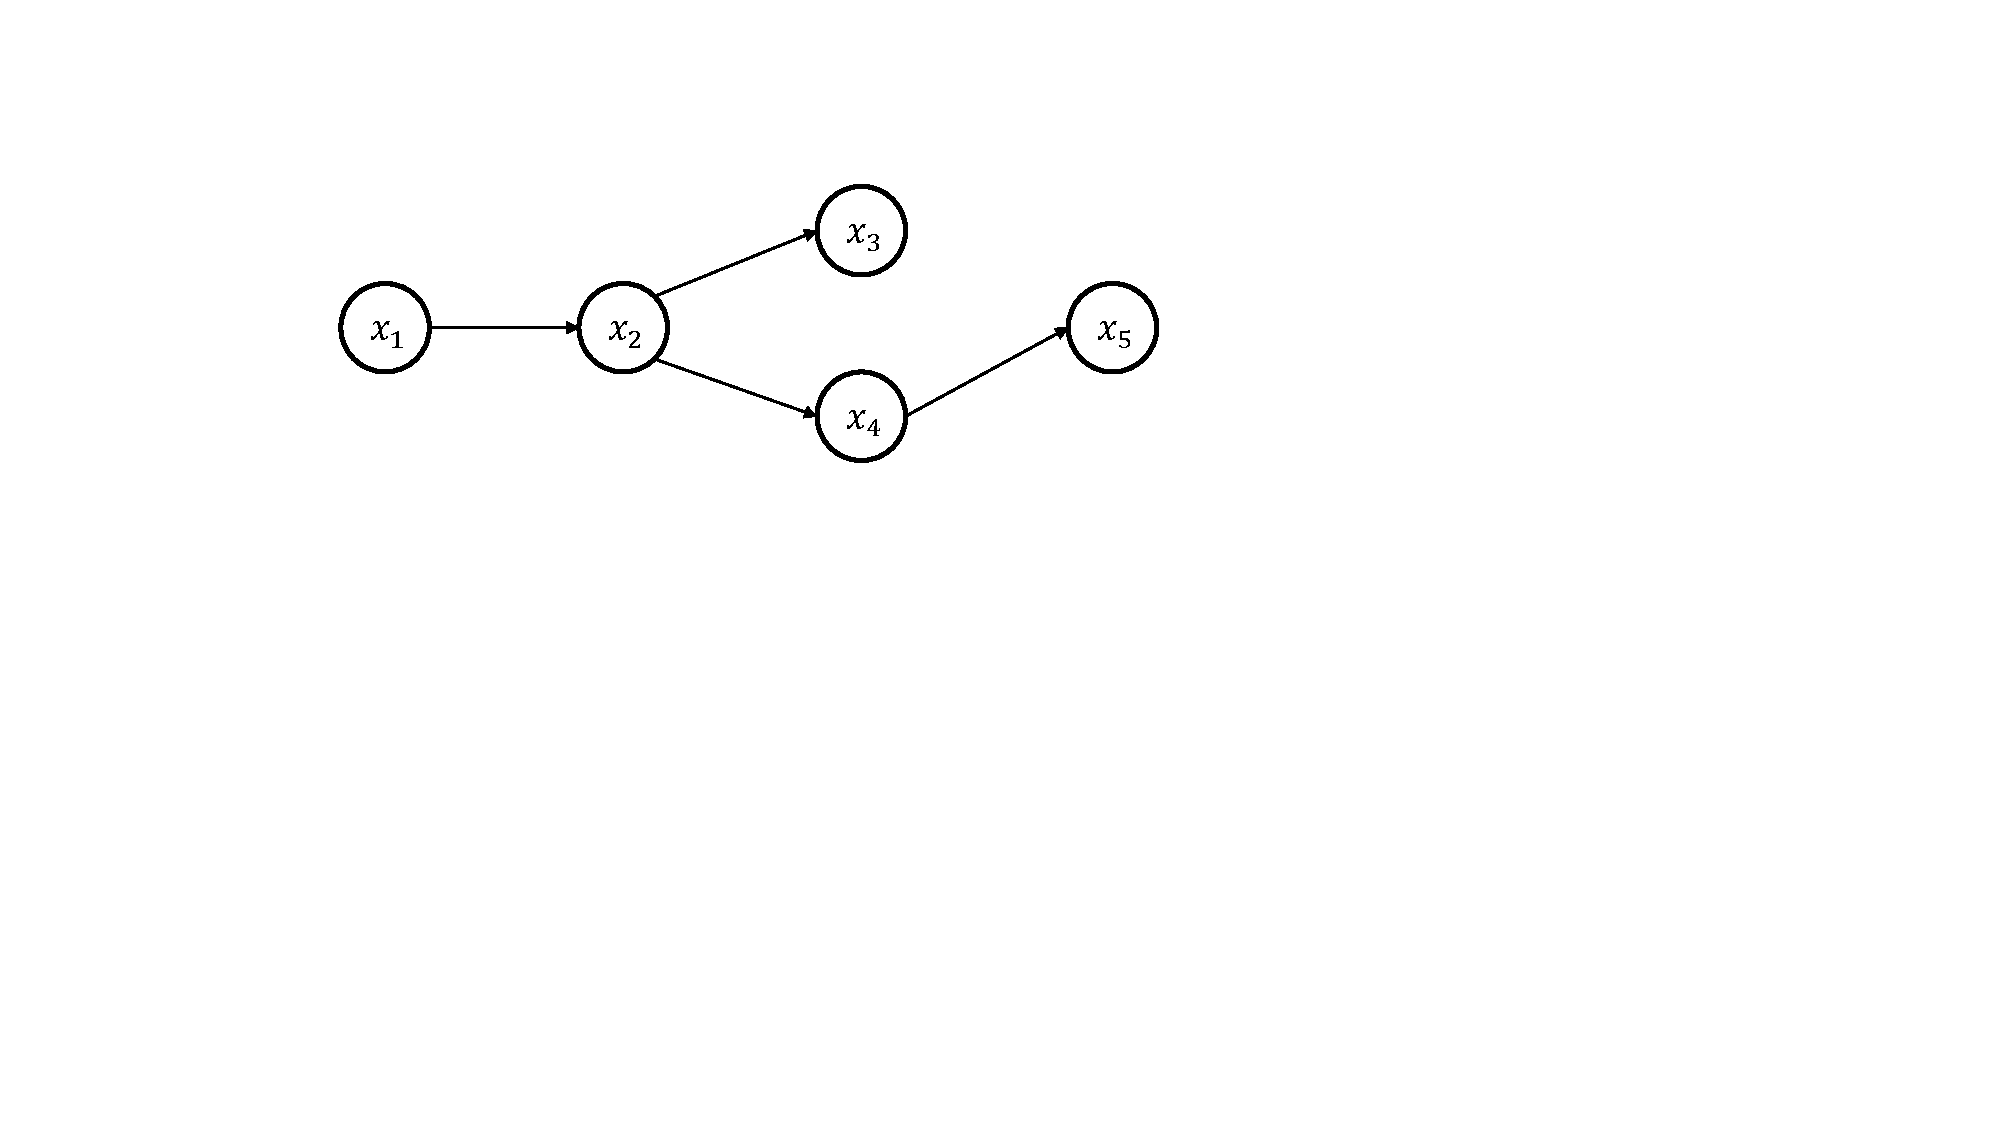
\includegraphics[width=0.65\linewidth]{dag.pdf}}
    \caption{贝叶斯网络结构}
    \label{fig:dag}
    \end{figure}

\part [20]
    本题探究变分推断相关内容.我们利用教材中相同的设定,假设当前有N个变量$\{x_1, x_2, \ldots, x_N\}$}均依赖于其他变量z,所有能观察到的变量”的联合分布的概率密度函数是:
    \begin{align}
    p(\mathbf{x} \mid \Theta) = \prod_{i=1}^N \sum_{\mathbf{z}} p(x_i, \mathbf{z} \mid \Theta), 
    \end{align}

    而所对应的对数似然函数为:
    \begin{align}
    \ln p(\mathbf{x} \mid \Theta) = \sum_{i=1}^N \ln \left\{ \sum_{\mathbf{z}} p(x_i, \mathbf{z} \mid \Theta) \right\}, 
    \end{align}

    其中 $\mathbf{x} = \{x_1, x_2, \ldots, x_N\}, \Theta$ 是 $\mathbf{x}$ 与 $\mathbf{z}$ 服从的分布参数.

    我们的推断任务是求解$p(\mathbf{z} \mid \mathbf{x}, \Theta)$和$\Theta$.一种有效手段是基于最大化对数似然函数,对(2)式使用EM算法:在 E 步,根据 $t$ 时刻的参数 $\Theta^t$ 对 $p(\mathbf{z} \mid \mathbf{x}, \Theta^t)$ 进行推断,并计算联合似然函数 $p(\mathbf{x}, \mathbf{z} \mid \Theta)$;在 M 步,基于 E 步的结果进行最大化寻优,即对关于变量 $\Theta$ 的函数 $Q(\Theta; \Theta^t)$ 进行最大化从而求取:
    \begin{align}
    \Theta^{t+1} &= \arg\max_{\Theta} Q(\Theta; \Theta^t) \\
    &= \arg\max_{\Theta} \sum_{\mathbf{z}} p(\mathbf{z} \mid \mathbf{x}, \Theta^t) \ln p(\mathbf{x}, \mathbf{z} \mid \Theta).
    \end{align}

    (1)(10 points)$p(\mathbf{z} \mid \mathbf{x}, \Theta^t)$未必是隐变量 $\mathbf{z}$ 服从的真实分布,而只是一个近似分布.现在将这个近似分布用 $q(\mathbf{z})$ 表示,请尝试验证
    \begin{align}
    \ln p(\mathbf{x}) = \mathcal{L}(q) + KL(q \parallel p), 
    \end{align}
    其中
    \begin{align}
    \mathcal{L}(q) = \int q(\mathbf{z}) \ln \left\{ \frac{p(\mathbf{x}, \mathbf{z})}{q(\mathbf{z})} \right\} d\mathbf{z}, 
    \end{align}
    \begin{align}
    KL(q \parallel p) = -\int q(\mathbf{z}) \ln \left\{ \frac{p(\mathbf{z} \mid \mathbf{x})}{q(\mathbf{z})} \right\} d\mathbf{z}.
    \end{align}

    (2)(10 points)假设复杂的多变量Z可拆解为一系列相互独立的多变量$Z_{i}$,即Z服从分布:
    \begin{align}
        q(\mathbf{z}) = \prod_{i=1}^M q_i(\mathbf{z}_i),
    \end{align}
    尝试从最大化$\mathcal{L}(q)$的角度说明变量子集 $\mathbf{z}_j$ 所服从的最优分布 $q_j^*$ 应满足
    \begin{align}
    \ln q_j^*(\mathbf{z}_j) = \mathbb{E}_{i \neq j}[\ln p(\mathbf{x}, \mathbf{z})] + \text{const}.
    \end{align}

\end{parts}

\begin{solution}
	\begin{parts}
            \part  对于这个题首先可以得到由联合概率分布求和的结果:
            \[
                P(x_5) = \sum_{x_4}\sum_{x_3}\sum_{x_2}\sum_{x_1}P(x_1,x_2,x_3,x_4,x_5)
            \]
            进一步推导得到:
            \[
                P(x_5) = \sum_{x_4}\sum_{x_3}\sum_{x_2}\sum_{x_1}P(x_1)P(x_2|x_1)P(x_3|x_2)P(x_4|x_2)P(x_5|x_4)
            \]
            所以根据书上说的,我们可以按照顺序计算加法,假设:$m_{ij}$代表的是求加过程的中间结果,下标i代表此项对于$x_i$求加的结果,j代表其他变量,
            则我们可以化简一些步骤例如:
            \[
                P(x_5) = \sum_{x_4}P(x_5|x_4)\sum_{x_3}P(x_3|x_2)\sum_{x_2}P(x_4|x_2)\sum_{x_1}P(x_1)P(x_2|x_1)
            \]
            其中比如:$\sum_{x_1}P(x_1)P(x_2|x_1) = m_{12}$,所以我们可以得到最终结果为:
            \[
                P(x_5) = m_{54}(x_5)
            \]
            具体其中的化简步骤可以一步一步推导来,比如:$m_{23} = \sum_{x_3}P(x_3|x_2) m_{12}$
            
            \part 
            (1).如果要证明这个公式,我们首先从基于$\boldsymbol{x}$的公式说起:
            \[
                p(\boldsymbol{x}) = \frac{p(\boldsymbol{x}, \boldsymbol{z})}{p(\boldsymbol{z}| \boldsymbol{x})}
            \]
            所以两边同时变换再除以$q(\boldsymbol{z})$:
            \[
                p(\boldsymbol{x}) = \frac{p(\boldsymbol{x}, \boldsymbol{z})/q(\boldsymbol{z})}{p(\boldsymbol{z}| \boldsymbol{x})/q(\boldsymbol{z})}
            \]
            然后取对数:
            \[
                \ln p(\boldsymbol{x}) = \ln \frac{p(\boldsymbol{x},\boldsymbol{z})}{q(\boldsymbol{z})} - \ln \frac{p(\boldsymbol{z}| \boldsymbol{x})}{q(\boldsymbol{z})}
            \]
            两边同时乘上$q(\boldsymbol{z})$,并且积分:
            \[
                \int q(\boldsymbol{z}) \ln p(\boldsymbol{x})\,d\boldsymbol{z} = \int q(\boldsymbol{z}) \ln  \frac{p(\boldsymbol{x},\boldsymbol{z})}{q(\boldsymbol{z})} \,d\boldsymbol{z} - \int q(\boldsymbol{z}) \ln \frac{p(\boldsymbol{z}| \boldsymbol{x})}{q(\boldsymbol{z})}\,d\boldsymbol{z}
            \]
            化简就得到了:
            \[
                \ln p(\boldsymbol{x}) = \int q(\boldsymbol{z}) \ln  \frac{p(\boldsymbol{x},\boldsymbol{z})}{q(\boldsymbol{z})} \,d\boldsymbol{z} - \int q(\boldsymbol{z}) \ln \frac{p(\boldsymbol{z}| \boldsymbol{x})}{q(\boldsymbol{z})}\,d\boldsymbol{z}
            \]
            这个式子的形式就是上面所示:
            \[
                \ln p(\boldsymbol{x}) = L(q) + KL(q || p)
            \]
            (2).因为要从最大化L(q)的角度来说明这个问题,我们把L(q)拿出来:
            \[
                L(q) = \int q(\boldsymbol{z}) \ln  \frac{p(\boldsymbol{x},\boldsymbol{z})}{q(\boldsymbol{z})} \,d\boldsymbol{z} 
            \]
            化简利用题目中条件可以得到:
            \[
                L(q) = \int \prod_{i = 1}^{M}q_i(\boldsymbol{z}_i) \{ \ln p(\boldsymbol{x}, \boldsymbol{z}) - \ln \prod_{i =1}^{M}q_i(\boldsymbol{z}_i)\}\,d\boldsymbol{z} 
            \]
            \[
                L(q) = \int \prod_{i = 1}^{M}q_i(\boldsymbol{z}_i)\ln p(\boldsymbol{x}, \boldsymbol{z}) - \prod_{i = 1}^{M}q_i(\boldsymbol{z}_i)\ln \prod_{i =1}^{M}q_i(\boldsymbol{z}_i)\,d\boldsymbol{z} = L_1(q) + L_2(q)
            \]
            先看第一部分:
            \[
                L_1(q) = \int \prod_{i = 1}^{M}q_i(\boldsymbol{z}_i)\ln p(\boldsymbol{x}, \boldsymbol{z}) = 
                \int q_j \{ \int \ln p(\boldsymbol{x}, \boldsymbol{z}) \prod_{i\neq j}^{M}(q_i(\boldsymbol{z}_i)d\boldsymbol{z_i})\} d\boldsymbol{z_j}
            \]
            令第一部分的$\ln \hat{p}(\boldsymbol{x}, \boldsymbol{z_j}) = \int \ln p(\boldsymbol{x}, \boldsymbol{z}) \prod_{i\neq j}^{M}(q_i(\boldsymbol{z}_i)d\boldsymbol{z_i})$,则原式子等于:
            \[
                L_1(q) = \int q_j \ln \hat{p}(\boldsymbol{x}, \boldsymbol{z_j})\, d\boldsymbol{z_j}
            \]
            对于第二部分
            \[
                L_2(q) = \int \prod_{i = 1}^{M}q_i(\boldsymbol{z}_i)\ln \prod_{i =1}^{M}q_i(\boldsymbol{z}_i)\,d\boldsymbol{z} 
                = \sum_{i1 = 1}^{M} \int \prod_{i2 = 1}^{M} q_{i2}(\boldsymbol{z_{i2}}) \ln q_{i1}(\boldsymbol{z_{i1}})  \,d\boldsymbol{z}
            \]
            令i1 = j,则$\int \prod_{i2 = 1}^{M} q_{i2}(\boldsymbol{z_{i2}}) \ln q_{i1}(\boldsymbol{z_{i1}})  \,d\boldsymbol{z} = \int q_j(\boldsymbol{z_j}) \ln q_j(\boldsymbol{z_j})\,d\boldsymbol{z_j}$,则式子二可以化简为:
            \[
                L_2(q) = \int q_j(\boldsymbol{z_j}) \ln q_j(\boldsymbol{z_j})\,d\boldsymbol{z_j} + const
            \]
            所以L(q)可以表示为:
            \[
                L(q) = -KL(q_j || \hat{p}(\boldsymbol{x}, \boldsymbol{z_j})) + const
            \]
            当且仅当,$q_j = \hat{p}(\boldsymbol{x}, \boldsymbol{z_j})$时,KL散度最小,此时估计值最近似。为了证明它满足这个分布,我们看之前得到的一个式子
            \[
                \int q_j \{ \int \ln p(\boldsymbol{x}, \boldsymbol{z}) \prod_{i\neq j}^{M}(q_i(\boldsymbol{z}_i)d\boldsymbol{z_i})\} d\boldsymbol{z_j} = \int q_j  \mathbb{E}_{i \neq j}[\ln p(\mathbf{x}, \mathbf{z})] \,d\boldsymbol{z_j}
            \]
            \[
                = \int q_j \hat{p}(\boldsymbol{x}, \boldsymbol{z_j}) \,d \boldsymbol{z_j} - const
            \]
            所以:
            \[
                \ln q_j^*(\mathbf{z}_j) = \ln  \hat{p}(\boldsymbol{x}, \boldsymbol{z_j})  = \mathbb{E}_{i \neq j}[\ln p(\mathbf{x}, \mathbf{z})] + \text{const}.
            \]
            则证明了,从最大化L(q)的角度来说,子集$z_j$的最优分布满足上述条件。
	\end{parts}
\end{solution}



\question [60] \textbf{强化学习}


\begin{parts}
\part [25] 
    价值迭代的更新公式为:

    \begin{align}
            V^{k+1}(s)=\max _{a \in \mathcal{A}}\left\{r(s, a)+\gamma \sum_{s^{\prime} \in \mathcal{S}} P\left(s^{\prime} \mid s, a\right) V^k\left(s^{\prime}\right)\right\},
    \end{align}

    其中$s$表示$t$时刻的状态,$s'$表示$t+1$时刻的状态,$a$表示$t$时刻的动作,$\gamma$是折扣因子.我们将其定义为一个贝尔曼最优算子 $\mathcal{T}$ :

    \begin{align}
        V^{k+1}(s)=\mathcal{T} V^k(s)=\max _{a \in \mathcal{A}}\left\{r(s, a)+\gamma \sum_{s^{\prime} \in \mathcal{S}} P\left(s^{\prime} \mid s, a\right) V^k\left(s^{\prime}\right)\right\}
    \end{align}

    若 $O$ 是一个算子,如果满足 $\left\|O V-O V^{\prime}\right\|_q \leq\left\|V-V^{\prime}\right\|_q$ 条件,则我们称 $O$ 是一个压缩算子,其中 $\|x\|_q$ 表示 $x$ 的 $L_q$ 范数.

    (1)(15 points)请证明,当 $\gamma<1$ 时,贝尔曼最优算子 $\mathcal{T}$ 是一个 $\gamma$-压缩算子.(提示:证明$\left\|\mathcal{T} V-\mathcal{T} V^{\prime}\right\|_{\infty} \leq \gamma\left\|V-V^{\prime}\right\|_{\infty}$即可  )

    (2)(10 points)在(1)的基础上,请说明价值迭代的收敛性.(提示:可以设最优价值函数为$V^*$,考虑$\left\|V^k-V^*\right\|_{\infty}$与迭代次数$k$的联系)
    
\part [15]
    本题探究蒙特卡罗强化学习算法中的策略.

    (1)(8 points)请你描述\textbf{重要性采样}的过程.具体来说,我们希望估计某个函数 $f(x)$ 在概率分布 $p(x)$ 下的期望,但是$p(x)$采样困难.如何引入一个更容易采样的分布 $q(x)$来协助估计?


    (2)(7 points)同策略蒙特卡罗强化学习算法和异策略蒙特卡罗强化学习算法有何差异?请你结合 
     上一问中提到的方法进行讨论.

\part [20]
    时序差分学习(TD学习)是一种在强化学习中广泛应用的核心技术,结合了动态规划和蒙特卡洛方法的优点,用于估计策略的价值函数.它通过直接从与环境的交互中学习,既不需要完整的模型,也无需等待整条轨迹结束即可更新估计.这种特性使TD学习在在线学习和实时决策任务中非常高效.教材中介绍了一种属于TD学习的经典算法-Sarsa算法,下方为完整算法流程:
    
    \begin{figure}[h!]
    \centerline{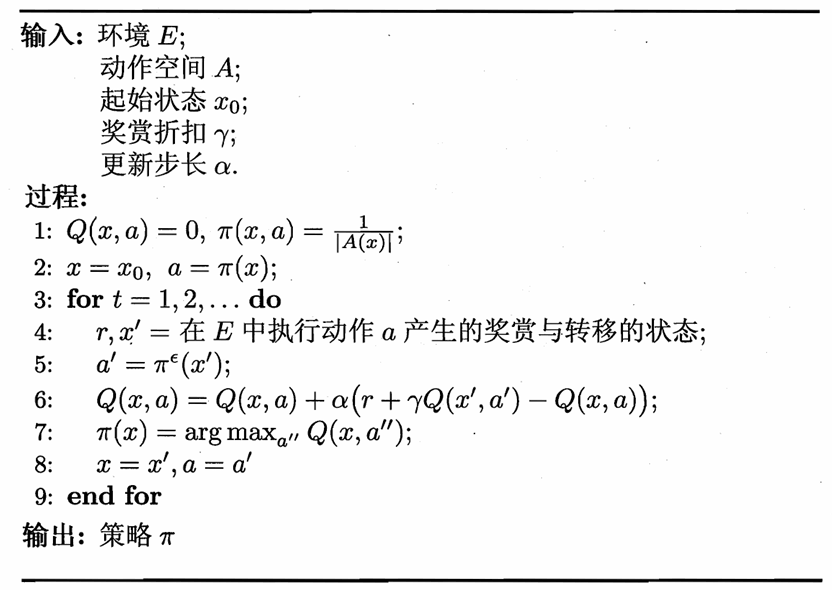
\includegraphics[width=0.65\linewidth]{image.png}}
    \caption{Sarsa算法}
    \label{fig:sarsa}
    \end{figure}

    \newpage
    结合状态值函数与状态-动作值函数的关系以及动态规划的特点,我们可以得到:
    \begin{align}
    Q^\pi(x, a) &= \sum_{x' \in X} P^a_{x \to x'} \left( R^a_{x \to x'} + \gamma V^\pi(x') \right) \\
    &= \sum_{x' \in X} P^a_{x \to x'} \left( R^a_{x \to x'} + \gamma \sum_{a' \in A} \pi(x', a') Q^\pi(x', a') \right).
    \end{align}

    请你根据式(15),(16),尝试推理出Sarsa算法的更新公式,即图二中的步骤6.


\end{parts}

\begin{solution}
\begin{parts}
	\part
	\part
        \part
\end{parts}
\end{solution}





\end{questions}

\end{document}